\documentclass{article}
\usepackage[a4paper]{geometry}
\usepackage{parskip}
\usepackage[colorlinks=true,linkcolor=black,urlcolor=blue]{hyperref}
\usepackage{amsmath}
\usepackage{tikz}
\urlstyle{same}
\date{}
\author{Sunaina Pai}

\title{Triangular Area}
\begin{document}
\maketitle

\section*{Problem}
In \( \triangle ABC \), produce a line from \( B \) to \( AC \), meeting
at \( D \), and from \( C \) to \( AB \), meeting at \( E \).  Let \( BD
\) and \( CE \) meet at \( X \). Let \( \triangle BXE \) have area \( a
\), \( \triangle BXC \) have area \( b \), and \( \triangle CXD \) have
area \( c \).  Find the area of quadrilateral \( AEXD \) in terms of \(
a \), \( b \), and \( c \).

Source: \url{http://www.qbyte.org/puzzles/puzzle01.html#p2}

\section*{Solution}
Draw a line segment \( AX \). Let the area of \( \triangle AXE \) be \(
x \) and the area of \( \triangle AXD \) be \( y \). We need to find \(
x + y \) in terms of \( a \), \( b \), and \( c \).

Extend the line segments \( CE \) and \( BD \) such that \( BH \) meets \( CE
\) and \( CG \) meets \( BD \) at right angles.

\begin{figure}[htbp]
\centering
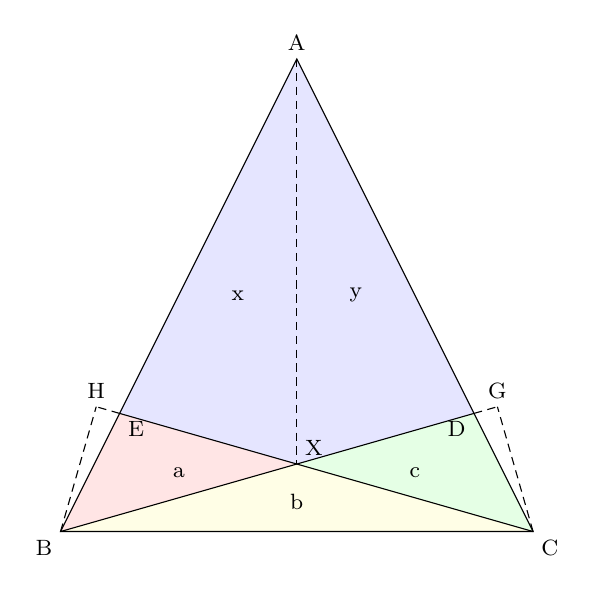
\begin{tikzpicture}[scale=1.5]
\footnotesize
\coordinate (A) at (2,4);
\coordinate (B) at (0,0);
\coordinate (C) at (4,0);
\coordinate (D) at (3.5, 1);
\coordinate (E) at (0.5, 1);
\coordinate (H) at (16/53, 56/53);
\coordinate (G) at (4-16/53, 56/53);
\coordinate (X) at (2, 4/7);

\filldraw[draw=none,fill=red!10] (B) -- (E) -- (X) -- cycle;
\filldraw[draw=none,fill=green!10] (C) -- (D) -- (X) -- cycle;
\filldraw[draw=none,fill=yellow!10] (B) -- (C) -- (X) -- cycle;
\filldraw[draw=none,fill=blue!10] (A) -- (E) -- (X) -- (D) -- cycle;

\node[above] at (A) {A};
\node[below left] at (B) {B};
\node[below right] at (C) {C};
\node[below left] at (D) {D};
\node[below right] at (E) {E};
\node[above] at (H) {H};
\node[above] at (G) {G};
\node[above right] at (X) {X};

\node at (2, 0.25) {b};
\node at (1, 0.5) {a};
\node at (3, 0.5) {c};
\node at (1.5, 2) {x};
\node at (2.5, 2) {y};

% AB: y = 2x; AC: -2x + 8
% BD: y = 2x/7; CE; -2x/7 + 8/7
\draw (A) -- (B) -- (C) -- cycle;
\draw (B) -- (D);
\draw (C) -- (E);

% BH: 7x/2
\draw[densely dashed] (B) -- (H);
\draw[densely dashed] (E) -- (H);
\draw[densely dashed] (C) -- (G);
\draw[densely dashed] (D) -- (G);
\draw[densely dashed] (A) -- (X);

\end{tikzpicture}
\end{figure}


We know that the triangles with collinear bases have a common height and
also their areas are in the ratio of their respective bases that are
collinear.

From \( \triangle BXE \) and \( \triangle BXC \) we have
\begin{align*}
\frac{EX}{CX} = \frac{a}{b}.
\end{align*}

From \( \triangle BXC \) and \( \triangle CXD \) we have
\begin{align*}
\frac{BX}{DX} = \frac{b}{c}.
\end{align*}

From \( \triangle AXB \) and \( \triangle AXD \) we have
\begin{align}
\frac{BX}{DX} = \frac{a + x}{y}
& \implies \frac{b}{c} = \frac{a + x}{y} \nonumber \\
& \iff              by = cx + ac. \label{eq1}
\end{align}

From \( \triangle AXE \) and \( \triangle AXC \) we have
\begin{align}
\frac{EX}{CX} = \frac{x}{y + c}
& \implies \frac{a}{b} = \frac{x}{y + c} \nonumber \\
& \iff              bx = ay + ac. \label{eq2}
\end{align}

Substituting \eqref{eq2} in \eqref{eq1} we get
\begin{align}
by = c \left( \frac{ay + ac}{b} \right) + ac
& \iff b^2y - acy = ac^2 + abc \nonumber \\
& \iff y = ac \left( \frac{b + c}{b^2 - ac} \right). \label{eq3}
\end{align}

Substituting \eqref{eq1} in \eqref{eq2} we get
\begin{align}
bx = a \left( \frac{cx + ac}{b} \right) + ac
& \iff b^2x - acx = a^2c + abc \nonumber \\
& \iff x = ac \left( \frac{a + b}{b^2 - ac} \right). \label{eq4}
\end{align}

Adding \eqref{eq3} and \eqref{eq4} we get the area of quadrilateral \(
AEXD \) as
\[
x + y = ac \left( \frac{b + c}{b^2 - ac} \right) +
        ac \left( \frac{a + b}{b^2 - ac} \right)
      = ac \left( \frac{a + 2b + c}{b^2 - ac} \right).
\]
\end{document}
